\documentclass[english]{cpp-hmwk}
   \usepackage{blindtext}

\begin{document}
\Homework{Lindenmayer systems - a C++ implementation}{Steffen Knoblauch}

\begin{abstract}
Lindenmayer Systems, short L-systems, are the result of \textbf{research from Lindenmayer et al.}\footnote{ZITIEREN} about the geometric features of plants.
L-systems are a concept to mathematicaly/formal describe and model the growth processes of plant development. They are not only restricted to the plant based developments, but can also be used to generate fractals.

L-systems have an inital state and use rules, like a formal grammar, to transform or rather rewrite the current state to create the next state of the development from a plant or a fractal.
It is therefore possible to successive calculate each state of the development.
Such a state of a L-system can be interpreted as commands for a turtle graphic, which creates the opportunity to draw the created fractals or plant states. 

Goal of this paper is to design an architecture for L-systems, which includes an implementation for L-systems, their creation and an interface for a turtle graphic. The interface should enable the polymorphic use of different turtle graphic implementations and enable drawing of the L-system state.
\end{abstract}

\pagebreak
\section{Introduction}
L-systems are a formal way to describe plant or fractal development and interpret the result as a graphic. In order provide a general understanding of Lsystems is this  paper organised in several topics. Section \ref{section:lindenmayer} is a short introduction to the general idea,  based around object rewriting, the grammar of L- systems and the interpretation of a L-system as graphic.
After discussing the architecture and possible implementation steps, a final concept for an implementation is proposed.The code for this implementation is available via my github repository.\footnote{https://github.com/frozzenshooter/LSystems}

Finaly, there is a conclusion and an outlook for possible future extensions.

\section{Lindenmayer systems}
\label{section:lindenmayer}
\subsection{History}
\label{section:history}
''[L-systems] were introduced in 1968 by Lindenmayer as a theoretical framwork for studying the development of simple multicellular organisms [...]''\footnote{Zitiert ausd abop Preface - Abschnitt Modeling of Plants} and were later used in computer graphics to generate visuals of organisms and fractals.

On the beginning the focus of L-systems theory was based on larger plant parts and the graphical interpretation used chains of rectangles to display a L-system. Further research into L-system extended the interpretations, resulting in a interpretation of a L-system state with a LOGO-style Turtle. These extension make it possible to model more complex plants and fractaals and display them in a graphical way. \footnote{Zitat abop Vgl. Seite 6 Chapter 1.3}

\subsection{General idea}
\label{section:gerneralidea}
The general idea of a L-system is the use of a rewriting system based on a formal grammar. The shape of a plant or a fractal consists of geometric pieces, for example a branch of a tree has several subbranches. ''When each piece of a shape is geometrically similar to the whole, both the shape and the cascade that generate it are called self-similar.''\footnote{Zitate The Nature of....  chapter 6 page 34 } The self-similartiy makes it possible to create a formal description for the plant or fractal generation as a formal grammar, further discussed in  section \ref{section:grammar}. The rewritng uses this formal description to generate the diffferent states of the development. ''In general, rewriting is a technique for defining complex objects by successively replacing parts of a simple initial object using a set of rewriting rules or productions.''\footnote{Zitiert von abop Chapter 1  - 1.1 Rewriting systems}. 

For example this concept can be used to rewrite a inital string, called axiom, with defined rewriting rules.
A simple example is the following grammar, which consits of only two nonterminals, A and B, and two production rules. 
The first rule is A\rightarrow AB, the second rule is B\rightarrow A. The arrow '\rightarrow' symbols the replacement, the rewriting, of the object on the left with the object of the right of the arrow.
The L-system has as axiom the value 'A' and will be expanded with these rules, creating the results in figure \ref{figure:simple_lsystem}.

\begin{figure}[h!]
	\centering
	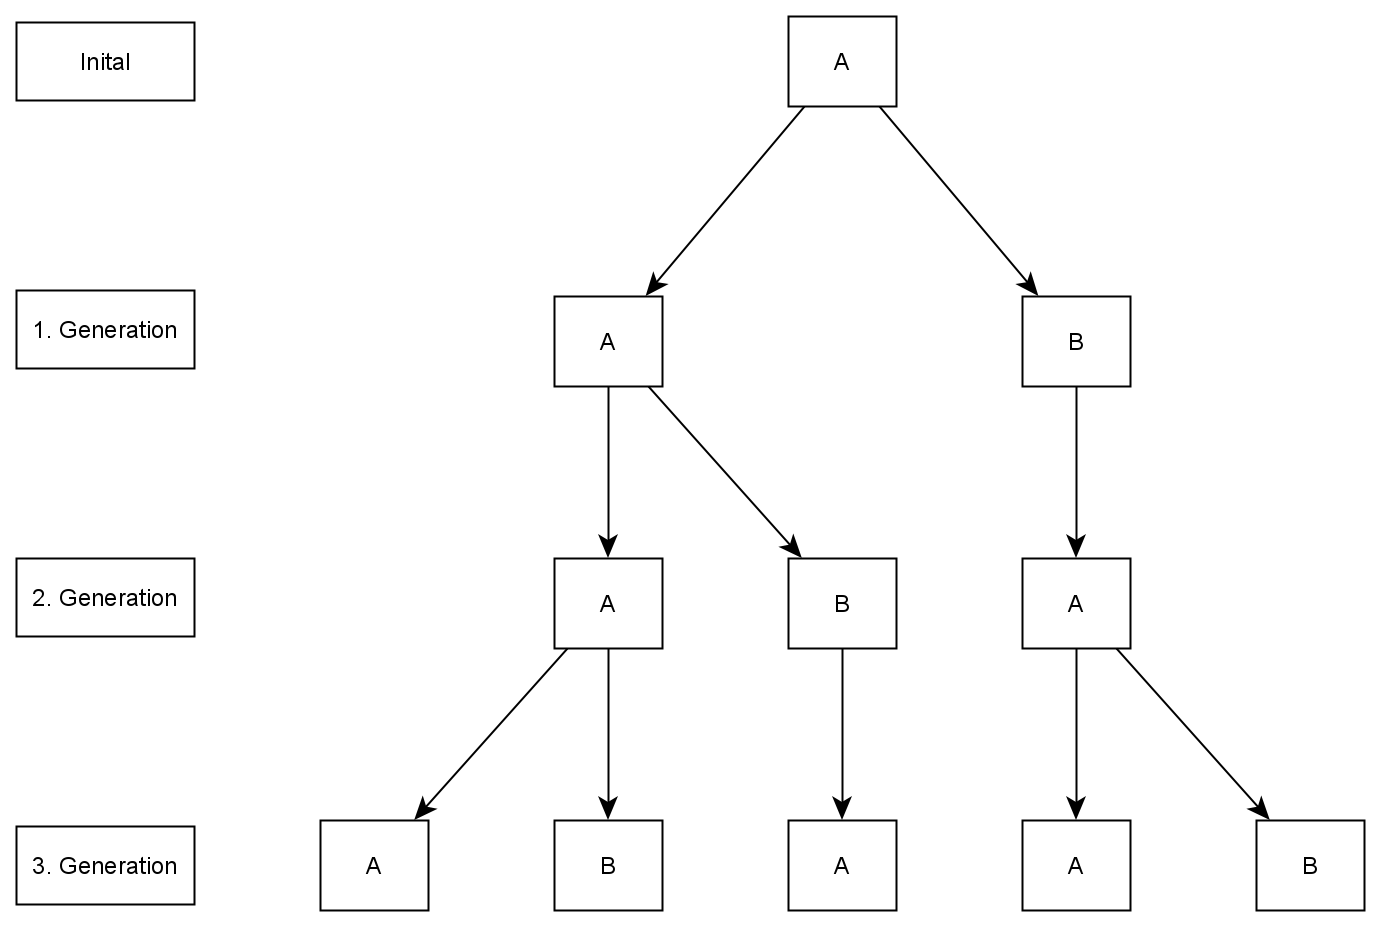
\includegraphics[width=0.7\columnwidth]{../graphs/Examples/simple_lsystem.png}
	\caption{Simple L-system}
	\label{figure:simple_lsystem}
\end{figure}

The first step is to use rule one, which replaces the nonterminal A with AB, resulting in the first generation. The result of the first generation ('AB') will be used to generate the second generation. For all nonterminals the productions will be parallel applied. In this case the nonterminals A and B will be replaced, because both have existing production rules. This results in the second generation with 'ABA' as result.

This process can be successively repeated recursive for a arbitrary amount of generations and create a fractal or plant with self-similar pieces. The more generations are calculated, the more detailed is the resulting state. 

\subsection{Grammar}
\label{section:grammar}
The definition of an L-system can be done similar to a Chomsky grammar, but there are some general differences. In Chomsky grammars the productions are applied sequentially, whereas in L-systems they can be applied parallel. This has some consequences for the formal properties of an L-system, for example a context-free L-system can produce a language which cannot be produced by a context-free Chomsky grammar.\footnote{Zitat abop vgl Seite 3  Abschnitt L-Systems}

\noindent This paper will only focus on a class of L-systems, the DOL-systems, which can be used for string based rewriting systems. This class is deterministic (D) and context-free (O) and can be formaly described  by a tuple:

\begin{center}
G = (V, $\omega$, P)
\end{center}

V: set of symbols as alphabet of the l-system - consiting of terminals and non terminals

$\omega$: axiom - nonempty word of the alphabet, which should contain at least one nonterminal

P: set of productions

\medskip
\noindent A production conistst of a predecessor, a nonterminal symbol of the alphabet, and a successor, the replacment of the nonterminal in the next generation.
To guarantee that the l-system is deterministic, there only can be one production for each nonterminal of the alphabet.The identity production is implicit a part of the set of productions.\footnote{Zitat vgl Seite 4 abop}

\medskip

If in the process of rewriting a terminal symbol is found, there will be no explicit production applied, but rather the identity production is applied. Terminals will therefore remain in future generations and won't extend an L-system with a production.

\medskip

\noindent As mentioned in section \ref{section:history} there are other extensions of a basic L-systems. The extensions introduce more possiblities for the generation process, like a non-deterministic behaviour. These extensions result in new grammars which can represent much complexer plants or fractals:

\begin{itemize}
\item Stochastic grammars: the system isn't deterministic anymore, because there can be multiple production rules for the same nonterminal with a probaility which results in a randomisation of the generation
\item Context senstive grammars: production not only look for the nonterminal, they rather look for the symbols bevor and after the current symbol to process, the context.
\item Parametric grammars: it is possible to set additional parameters for a symbol to influence the generation or the evaluation of the data
\end{itemize}

\subsection{Interpretation as turtle commands}
\label{section:turtle}
The L-systems introduced to this points are capable of creating a string based on a grammar. In order to create a graphic of a state of a L-system, the resulting state can be interpreted as commands of a turtle.

\noindent A turtle is a concept introduced by the language Logo as a tool for computer graphics.\footnote{Zitat VGL. Seite 179 Chappter 10 Logo book}

\noindent A state of a turtle can be described as a tuple\footnote{Zitat vgl abop Seite 6 ff}:

\begin{center}
S = (x,y, $\alpha$)
\end{center}

x and y are Cartesian coordinates

$\alpha$ is the direction in which a turtle is facing, called heading

\medskip

\noindent A turtle can move in the Cartesian coordinate system by altering the current state.You can think of it as a real turtle with a pen attached to it, walking on a paper. While moving in the coordinate system, or on the paper, the turtle can draw lines. Given this concept the turtle can receive different commands. The commands let the turtle walk on the paper or the coordinate system by altering the current state and drawing a line. For now I'll restrict this to a two dimensional coordinate system, but it is also possible to enhance it for a three dimensional coordinate system.

\medskip

\noindent The walking path of the turtle is controlled by commands. Therefore a defined step size \textit{d} and an angle \textit{$\theta$ } is needed to calculate the next state of the turtle.

\begin{itemize}
\item Draw: moves one step in the current facing direction drawing a line 
\item Move: moves one step in the current facing direction without drawing a line
\item Right-turn: turns to the right by the angle $\theta$
\item Left-turn: turns to the left by the angle $\theta$
\end{itemize}
\footnote{Zitat vlg cad book seitev 2 unteres drittel}

\noindent Additional to the state of the turtle the state there is a state for the pen. The pen state consist of the color and its width, which will result in more colorfull or different pictures.

\medskip

\noindent  With the given turtle concept is it possible to interpret the result of an L-system. Therefore a mapping between the symbols in the alphabet and the commands which should be called is needed.
This could be done by an arbitrary mapping between a nonterminal or a terminal and a command. For this paper the following mapping will be used, but the concept for the architecture includes the possibility to use other mappings in the future.

\noindent For the mapping alphabet V is used, which is a simple basic version of a L-system:

\begin{center}
V = (F, f, +, -)
\end{center}

This alphabet will be mapped with these turtle commands:

\begin{center}
\begin{tabular}{ c l }
Symbol & Turtle interpretation \\
\hline
F & Draw a line in the facing direction  \\ 
f & Move in the facing direction  \\  
+& Turn right  \\  
-& Turn left  \\  

\end{tabular}
\end{center}

This interpretation enables to draw the result of the L-system by iterating over every terminal and nonterminal of the result state and calling the mapped command. If no command is mapped the symbol will be skipped.

\subsection{Examples}
This section will present some examples for L-system grammars which create fractals. They were created with the implementation, described in section \ref{section:impl} under the use of the command mapping from section \ref{section:turtle}. 
\footnote{The grammars and further examples can be found under: \fullcite{examples1997}}
  
\subsubsection{Hilbert curve}
This fractal will be generated with the simple axiom 'L' and tow productions: 

\begin{itemize}
\item L\rightarrow +RF-LFL-FR+
\item R\rightarrow-LF+RFR+FL-
\end{itemize}


\noindent The turtle will be initalized with an angle of 90° and length \textit{d} of 5 for a step. The result is displayed in figure \ref{figure:Hilbert}.

\begin{figure}[h!]
	\centering
	
\includegraphics[width=0.6\columnwidth]{../graphs/Examples/hilbert.png}
	\caption{Hilbert L-system - 7 generations}
	\label{figure:Hilbert}
\end{figure}
 

\subsubsection{Sierpinski triangle}
This fractal will be created with 'F' as axiom and two productions:

\begin{itemize}
\item X\rightarrow YF+XF+Y
\item Y\rightarrow XF-YF-X
\end{itemize}

\noindent The turtle will be initalized with an angle of 60° and an arbitrary length \textit{d} for a step. The result is displayed in figure \ref{figure:Sierpinski}.
 
\begin{figure}[h!]
	\centering
	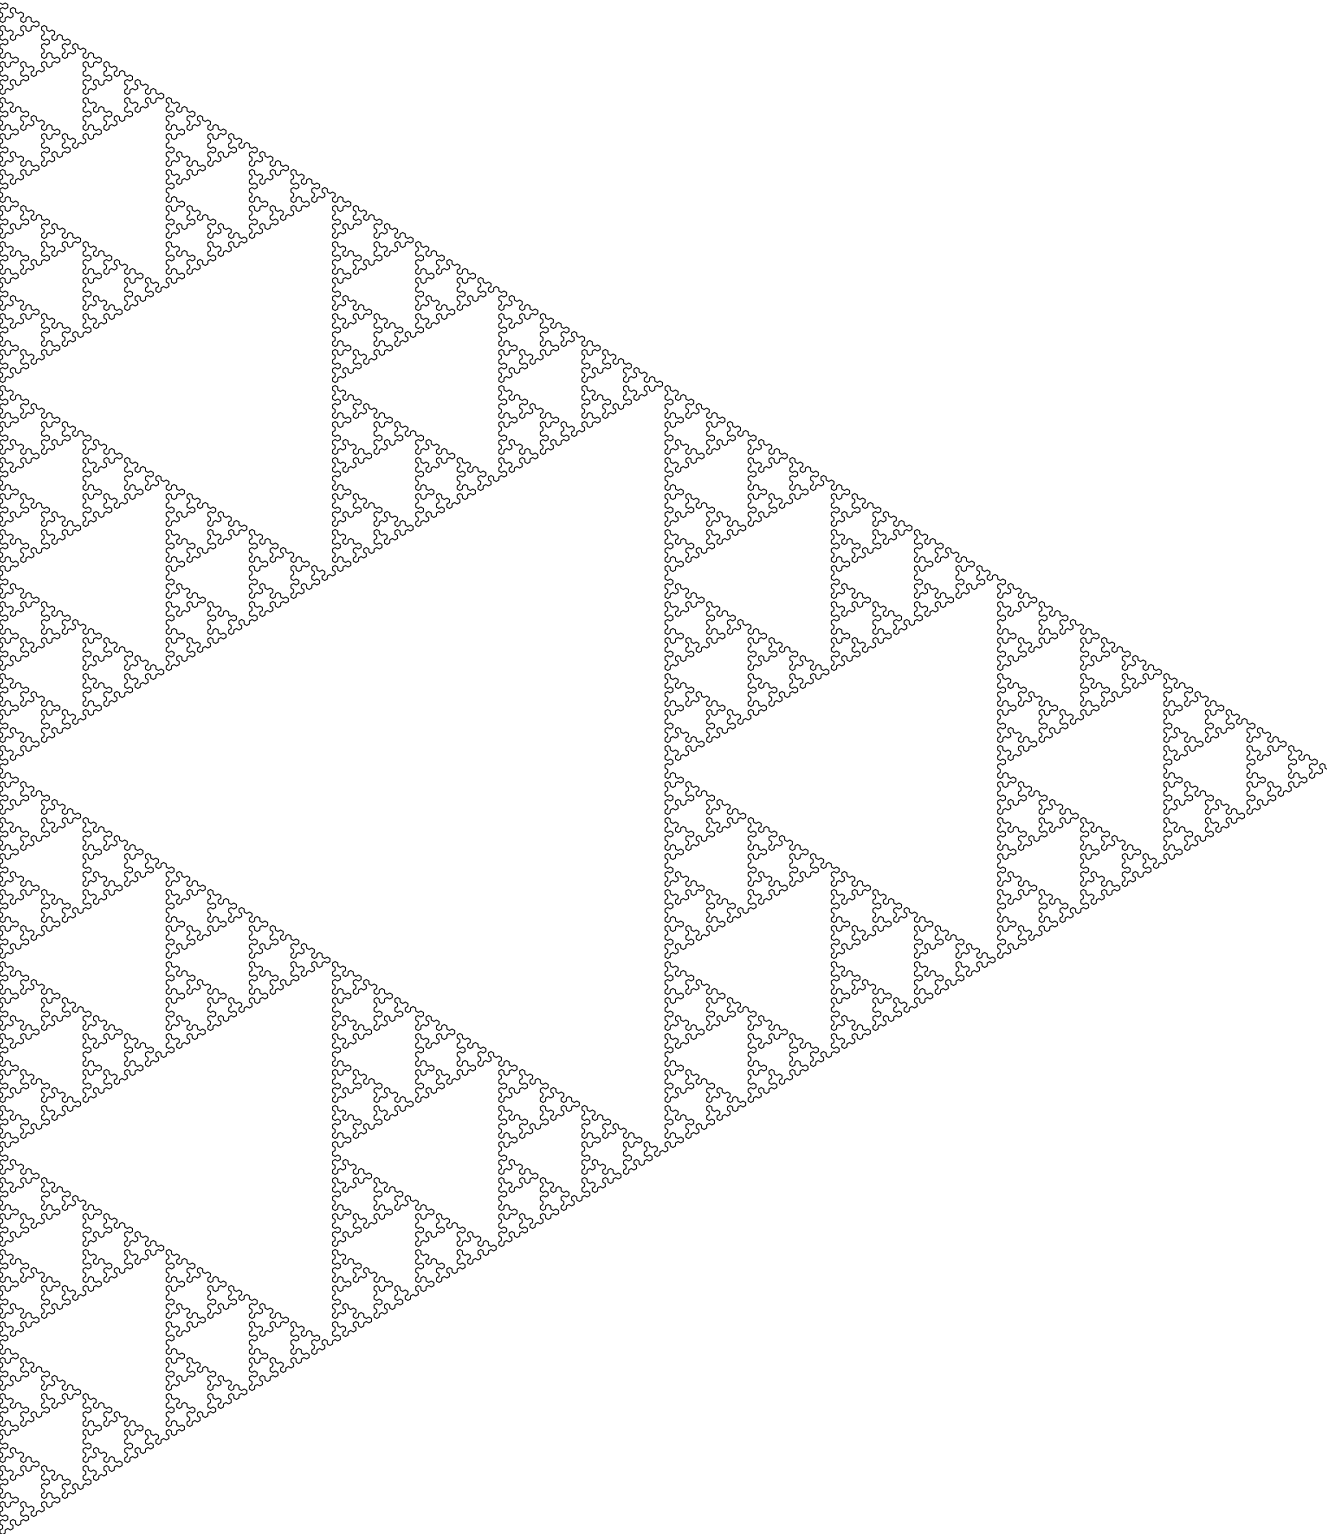
\includegraphics[width=0.6\columnwidth]{../graphs/Examples/sierpinski.png}
	\caption{Sierpinski L-system - 9 generations}
	\label{figure:Sierpinski}
\end{figure}
 

\clearpage
\section{Architecture}
The primary goal of this paper is creating an architecture and an implementation of a L-system as described in section \ref{section:lindenmayer}. The focus of the architecture will be on flexibility and expandability and therefore is the following section splitted into several parts with discussions about different aspects of the final architecture.

\footnote{HIER SOLLTE MAN EVT NOCH IRGENDWO DIE SEMANTSCIHE SCHNITTSTELLE ERWÄHNEN}

\subsection{Requirements overview}
The architecture for a L-system, as introduced in section \ref{section:lindenmayer}, has several requirements . This section will introduce the needed core requirements to get a flexible L-system and turtle.

\medskip
\noindent The core of the concept is the L-system itfself, which has to guarantee a flexible usage. The L-system holds relevant data like the grammar, consisting of production rules and an axiom. The L-system should offer a way to configure a grammmar and guarantee the usage in different architectures without hardcoded grammars. The L-system should also offer to successively generate the next states of the configured grammar and access this generated result.

\medskip

\noindent The turtle is another key component, which will be used to interpret the result of a L-system. The turtle has to offer the typical turtle commands as introduced in section \ref{section:turtle}. In order to provide a turtle that is as extensible as possible, it should be possible to implement it flexibly. Therefore an interface should be offered, that enables a fast exchange of implementations. Depending on the implementation of a turtle, it should be possible to configure the turtle and change properties, like the color or line width.

\medskip
\noindent A mapping between the turtle commands and the L-system alphabet is an important part, so it is possible to call the correct turtle commands. Additional a function which is calling the mapped commands, after interpreting the L-system result, is needed to create an image of a plant or a fractal development state.


\subsection{L-system}
\label{section:lsystem_discussion}
This section provides a dissussion of possible implementations of the L-system and a final proposal.

\medskip

\noindent A simple and rather naive idea would be an object which holds the L-system as a string and addtional the grammar, consisting of productions and an axiom. This L-system could offer a function that calculates the next generation by iterating over every char in the string. If there is a production for the current char, the char will be replaced according to the production with the successor. This function could be called for n generations to create the n-th generation of the L-system, as show in figure \ref{figure:naive_lsystem}.

\begin{figure}[h!]
	\centering
	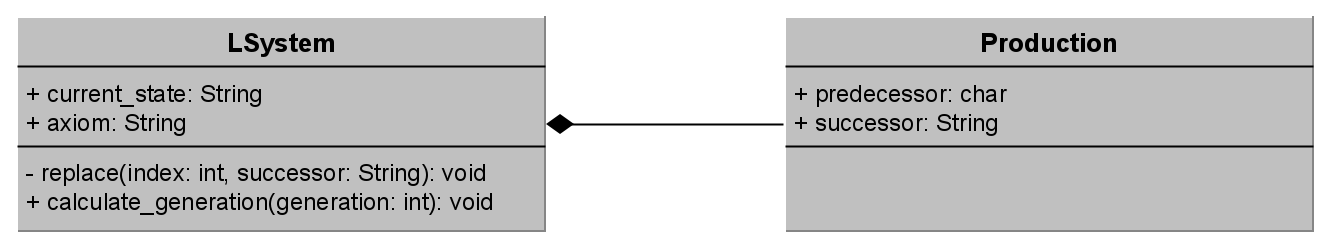
\includegraphics[width=1\columnwidth]{../graphs/LSystem/naive/class_diagram_l_system_naive.png}
	\caption{Naive L-system}
	\label{figure:naive_lsystem}
\end{figure}

\medskip
\noindent This idea has several design flaws resulting in a bad performance and unflexible architecture. The first flaws exist because of the lack of seperation between datastructure and processing of the data. It is not possible to simply exchange the datastructure or the function without the seperation, which affects flexibility of the L-system negative. This can be solved by extracting the functionality into a seperate function and the datastructure remains as ''dumb'' object. The seperated function can be a used to manipulate the current state in the datastrutcture itself and also creates the opportunity to exchange the underlying datastructure, as long as the datastructure fullfills some formal properties, like the support of access to the string and grammar.\newline
For a more flexible design additional changes could be done, because the current idea bases on chars as alphabet of the grammar. The L-system could be enhanced by allowing arbitrary objects as symbols of the alphabet, as long as they provide certain functions, like a operator to compare them. Instead of a string, the objects could for example be saved as a list.\newline
A further flaw is the bad performance, because of the use of a string to save the current state/generation. There are two reasons why the performance is bad, especially for larger generations. The first reason is the size of the string itself, which will grow very fast because of the nature of a L-system. Every nonterminal will be often replaced by severall symbols, which enormously increases the total size of the string for each generation. Additional to the large amount of space needed for the string, the replace in a string needs to be done for each nonterminal, which can result in a big overhead. Because of this problems, another more efficient design is needed.\newline
This implementation only works for simple L-systems where only a few generations are needed.

\medskip
\noindent In order to solve this problems and to create a more efficient and flexible architecture, let's recap the nature of L-systems. The generation of a L-system is based on a rewriting process. This process iterates over every object in the current state and calcualtes the resulting generation by applying the productions. Because of the restriction to DOL-systems, the rewriting is not context-sensitive and can be done independent from other objects of the current state. If a object gets replaced by the successor of the production, the result of this replacment can be handled independent. Consequently, the calculation of the n-th generation can be done for each object on their own and can simply be done in a recursive manner.\newline
There is only a limited number of productions in a grammar of a L-system. Each of these productions is choosen deterministic when comparing the current nonterminal with the predecessor. The next generation is created by rewriting the current state, when a nonterminal is often in the current state, the same production can be used. If the same production is used muliple times, the resulting generation has a lot of similar objects or more specific the same string muliple times. The repeating data and the recursive calculation can be used to improve the naive idea.

\medskip
\begin{figure}[h!]
	\centering
	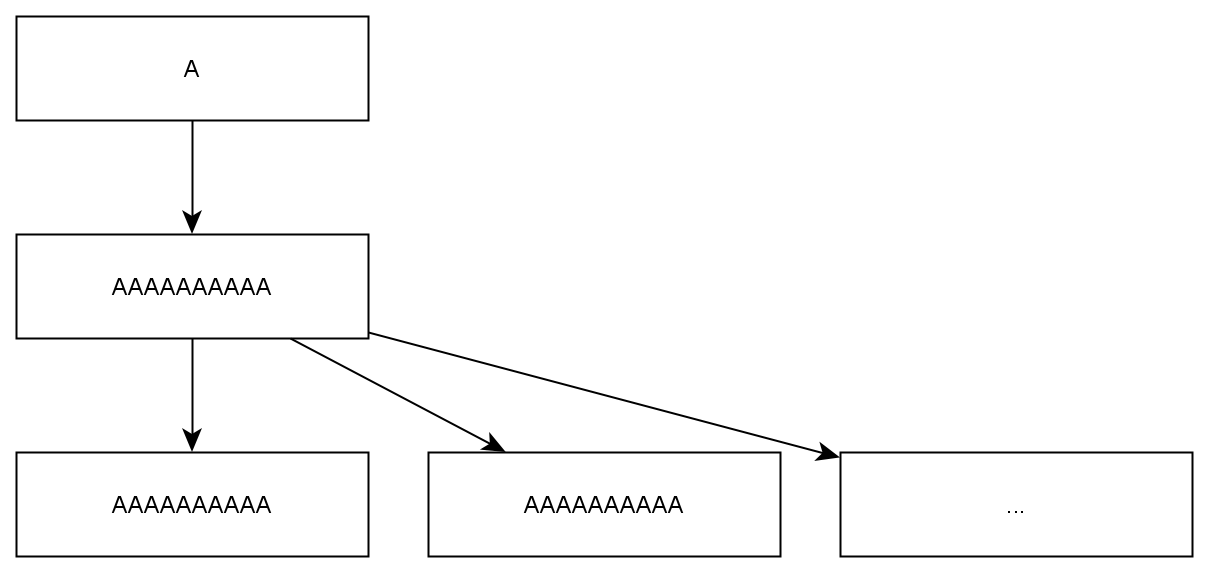
\includegraphics[width=0.8\columnwidth]{../graphs/LSystem/examples/simple_grammar_data_doubling.png}
	\caption{Memory reduction}
	\label{figure:lsystem_mem_reduction}
\end{figure}

\noindent The simple example in figure \ref{figure:lsystem_mem_reduction} shows the possible reduction of data using the following grammar:

Axiom: A

Production: A \rightarrow AAAAAAAAAA 

\medskip
\noindent This rather ideal example shows how it would be sufficient to save just parts of the resulting string to represent the whole generation of a L-system. For this example it could be possible to save ''AAAAAAAAAA'' and how often it is needed. Because of the repetitions, this is partly even for more complex grammars possible.

\medskip
\noindent With this knowledge multiple improvements can be discussed. The first possible improvement is storing the data not in a simple list, like a string, but instead in a more sophisticated datastructure. For this case a graph as datastructure is better suited. Such a graph enables a better performance for replacements and reduction of memory space.

\medskip
\noindent The graph has a special sturture to achive the improvements for a L-system. The following grammar is used to demonstrate the possible improvements:
 
Axiom: A

1. Production: A \rightarrow BBB

2. Production: B \rightarrow AAA

\medskip

\noindent A natural improvement of a graph is the replace function. This could be done by simply creating new childnodes with the replaced data. In figure \ref{figure:lsystem_graph} is a example with the given grammar. Each generation has its own nodes with data of the current state. A level of this graph represents a whole generation and can be accessed with the depth of the nodes.

\begin{figure}[h!]
	\centering
	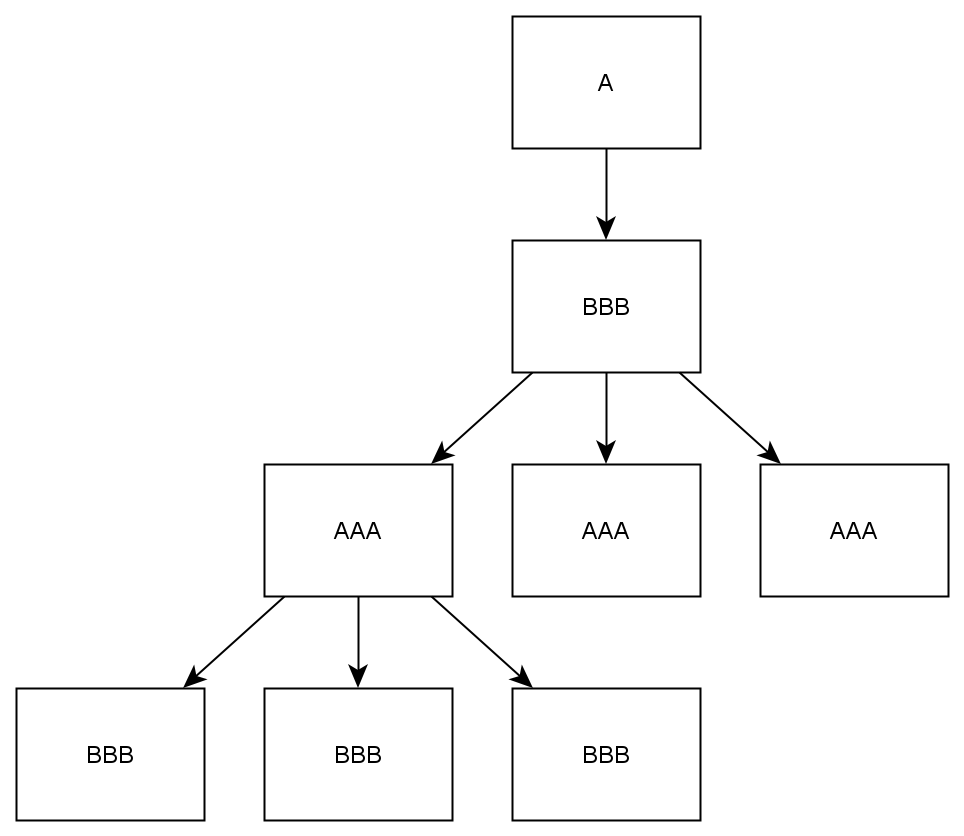
\includegraphics[width=0.8\columnwidth]{../graphs/LSystem/examples/lsystem_graph_example.png}
	\caption{L-system as graph}
	\label{figure:lsystem_graph}
\end{figure}

\medskip

\noindent This graph still has the problem of the redundant data, because every note contains its own data. For example in the second generation the part ''AAA'' is stored three times. This can be improved with another indirection of the data. This concept results in a datastructure containing a graph to store the dependencies and a container for the data itself. In figure \ref{figure:lsystem_graph_mem_reduction} is an example for this indirection. Each node saves a pointer or id of the data it represents. In this graph a replace could also be done with the creation of a childnodes.

\begin{figure}[h!]
	\centering
	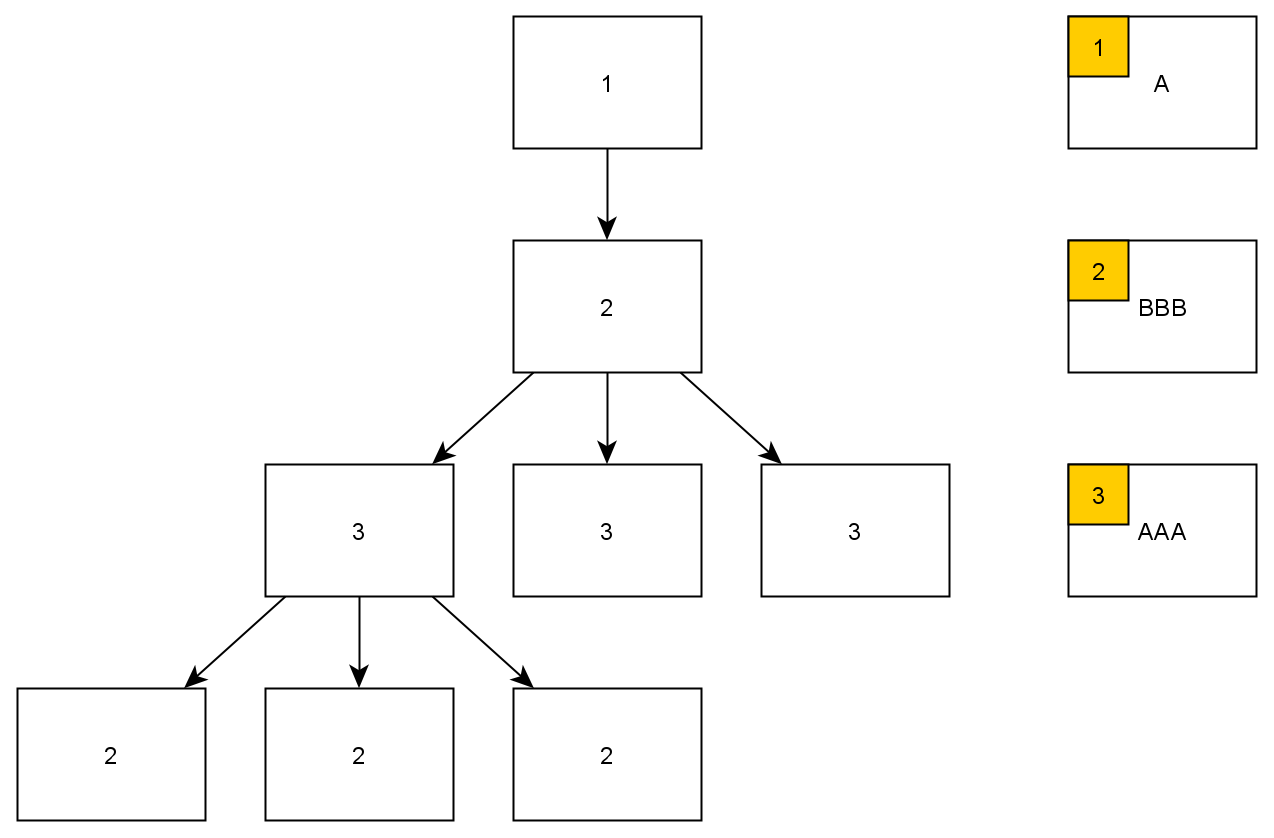
\includegraphics[width=0.8\columnwidth]{../graphs/LSystem/examples/lsystem_graph_reduced_example.png}
	\caption{L-system as graph with improved memory consumption}
	\label{figure:lsystem_graph_mem_reduction}
\end{figure}

\medskip
\noindent Both of the described graphs hold every calculated generation, which allows the access to an arbitrary generation with the restriction to the deepest calculated generation. To reduce the amount of storage needed even more, it is possible to neglect if all generations are needed or only the current generation. If only the last calculated generation is needed, the graph can be simplified even more. To discuss the simplification, it is necessary to look further in the different ways to do the replacement. It  is possible to iterate over the node data and replace for each symbol of teh data at a time. For example with the current grammar the data ''AAA'', could be replaced by replacing each ''A'' at a time. Because of the focus of DOL-Systems, another possible method is to replace a node with all childnodes at once.\newline
There seems to be no difference, but in combination with the proposed next step of the graph, it is relevant. If not all generations have to be stored, it is possible to remove a completely replaced parentnode. For example in figure \ref{figure:lsystem_graph_one_generation}, it is not needed to save the crossed out nodes, because they are completely replaced. In this simple example is it already possible save only four instead of six nodes and reduce the data. This results in a flat graph with only a few nodes depth, but only the current state of a L-system. For this graph, it is  important how the replacement is done. If the replacment is done with the all at once method, the parent node can be deleted directly. If the step by step replacement is done, it is nessecary to alter the parentnode data for each replacement. Only when the complete data and the parentnode is replaced, this node can be deleted. The complete replacement is simpler to implement, because the altering of parentnode data is not needed.

\begin{figure}[h!]
	\centering
	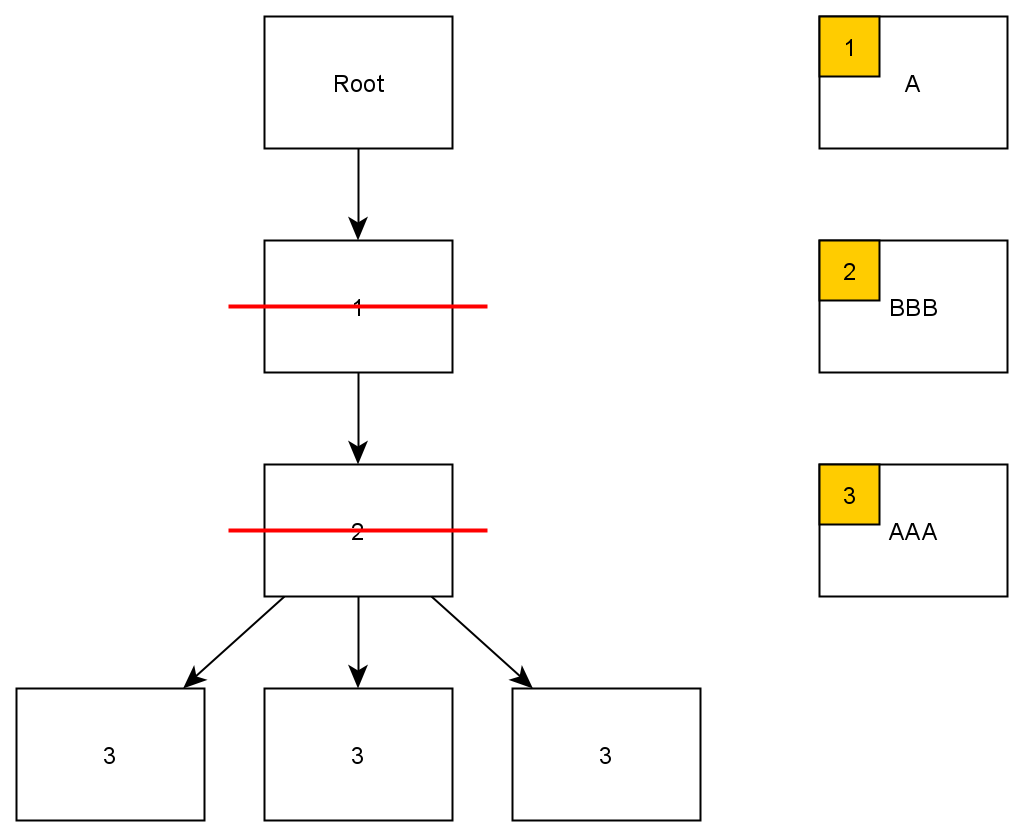
\includegraphics[width=0.8\columnwidth]{../graphs/LSystem/examples/lsystem_graph_reduced2_example.png}
	\caption{L-system as graph with one generation}
	\label{figure:lsystem_graph_one_generation}
\end{figure}

\medskip
\noindent A graph is as consequence a faster and memory saving approach in comparison to the naive L-system.

\bigskip

\noindent Another possible simplification is to neglect storing the generations of a L-system at all. Instead of saving the generation of a L-system in a datastructure, the result can be calculated on demand and never stored. The only data such a L-system would hold, would be the grammar itself. The calculation can be done with a recursive function, that will return the generation. Clearly an advantage is the reduction of needed storage space, but this reduction is only achived at the cost of recalculation for each generation. Whenever a generation is needed, it is nessecary to calculate again and it is not possible to use a previous result.
If a generation is needed multiple times or if it is needed to setp forwards and backwards in the result, a solution could be to store the result in another object. This calculations also guarantees a flexiblity, because you can either only calculate the generation once and use the result directly, like in this case to call the turtle commands, or save it for later usage.
 
The recursive function can be designed flexible in order to allow a simple exchange of a L-system datastructure. This results in two main components, the L-system datastructure and the function, which accepts a L-system datastructure and calculates the generation. The L-system, which the function receives, has to fullfill some requirements, like to offer access functions. This will be described in further detail in the implementation in section \ref{section:impl}.
 
\bigskip
 
\noindent There are the two possible ways to handle the L-system. The storage as a datastructure, based on a graph, and the recursive calculation. For this paper it is completely sufficient to calculate the generation on demand, because it is only necessary to call the turtle command once for each object of the L-system generation. As consequence no implementation of the graph is needed. Other use cases in the future might need to store the data. This would even be possible with the recursive function, when the result is stored in another object, for example a graph. The proposal for the L-system is shown in figure \ref{figure:lsystem_proposal}.

\begin{figure}[h!]
	\centering
	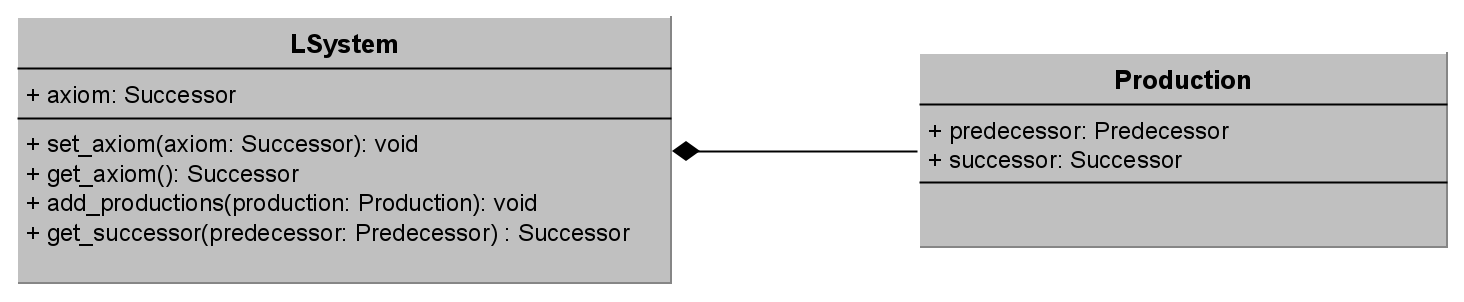
\includegraphics[width=1\columnwidth]{../graphs/LSystem/examples/l_system_proposal.png}
	\caption{L-system proposal}
	\label{figure:lsystem_proposal}
\end{figure}

\medskip
\noindent The proposed L-system will just hold the grammar for a L-system, which will be given to the recursive function. This L-system can be used in a flexible way, because it can be configured without a restriction of the grammar.Additonal, there is only a general type restriction for the axiom and the prodcutions. The types called Successor and Predeccessor can be choosen freely, but they need to fullfill formal requriements. The self-similarity and ergo the rewriting need to be represented by the types. The Successor type must consist of Successor objects itself, which can be splitted into objects of the Predecessor type. Each Predecessor object must be comparable to another Predecessor to be able to rewrite the L-system. 
 The type of the axiom and the successor have the same type, in order to guarantee that they are splittable in smaller parts.
 
To this point the discussion doesn't include how the turtle commands can be called. As already mentioned there must be mapping between the commands of turtle and the alphabet of the L-system. The mapping will be discussed further in section \ref{section:turtle_mapping} and for now we just asume a mapping exists in some way. When using a graph, it would be possible to call the turtle commands by accessing a generation data and interpret the objects.

Here the implementation is based on a recursive function. This function can call the turtle commands for a generation or more specific when the recursion depth is reached. How this will be done in detail is described in section \ref{section:impl}, but is based around the idea of an output iterator. The recursive function will receive an arbitrary output iterator and instead of interpreting the data in the function itself it will just hand over the objects of the generation to the iterator. This iterator can than interpret the objects as turtle commands and call them. The iterator has no restrictions on what to do with the data. For example the iterator may be used to save data in an arbitrary datastructure or print it in a file.

Overall allows this concept, consiting of the L-system datastructure and the recursive funtion, a possible user a flexible field of operation. The recursive function and the L-system datastructure can be used completely independent. For this concept, these components will be used together, in combination with other components, like a turtle and a turtle command mapping.

\subsection{Turtle}
A quiet important component of the architecture is the turtle. The turtle has to offer the typical commands as described in section \ref{section:turtle}. A turtle should be so flexible that it is possible to implement it for different Framworks, for example OpenGL or the Cairo graphics library. An abstract interface, with a minimal set of commands, will allow to implement this. A turtle like this is not only bound to a special graphics framework, but can be even implemented for other usecases, like generating text on the console or a file.
The most general or abstract version of a turtle offers the four minimal functions of a turtle, as shown in figure \ref{figure:minimal_turtle}.

\begin{figure}[h!]
	\centering
	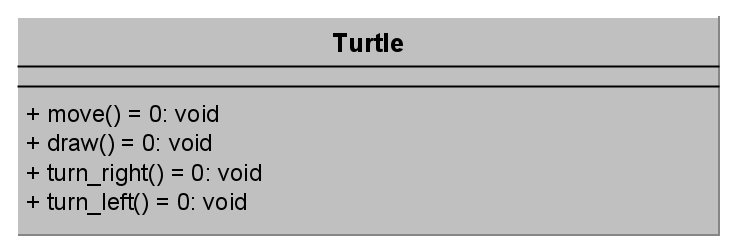
\includegraphics[width=0.6\columnwidth]{../graphs/LSystem/examples/class_simple_turtle.png}
	\caption{Minimal turtle}
	\label{figure:minimal_turtle}
\end{figure}

\medskip
\noindent More specialiced versions can offer more functions, depending on other needs and completly undependent of the paper usage of the turtle. For example an OpenGL implementation can offer more commands to represent a three dimensional turtle, like rotate around an axis. Additional to more commands, also different ways to configure a turtle can be offered for each specialization. Some possible implementations, in connection with this paper, will be described in section \ref{section:impl}.

Consequently the general interface is not only sufficient for this paper, but also for other usecases in the future.

\subsection{Turtle command mapping}
\label{section:turtle_mapping}
It is nessecary to map a command to an object in order to interpret the result of a L-system. As mentioned in section \ref{section:lsystem_discussion} a recursive function will be used to calculate the result of a L-system. Until this point we just assumed there was a mapping between the members of the alphabet of the L-system and the commands which will be called. In this scenario the recursive functionreceives an iterator which can handle the generated data. 
The command mapping iterator is a simple output iterator, which will handle calls of the turtle commands. In figure \ref{figure:if_command_map} is the general concept of the iterator displayed. The output iterator receives data, interprets it according to the mapping and calls the specified command.

\begin{figure}[h!]
	\centering
	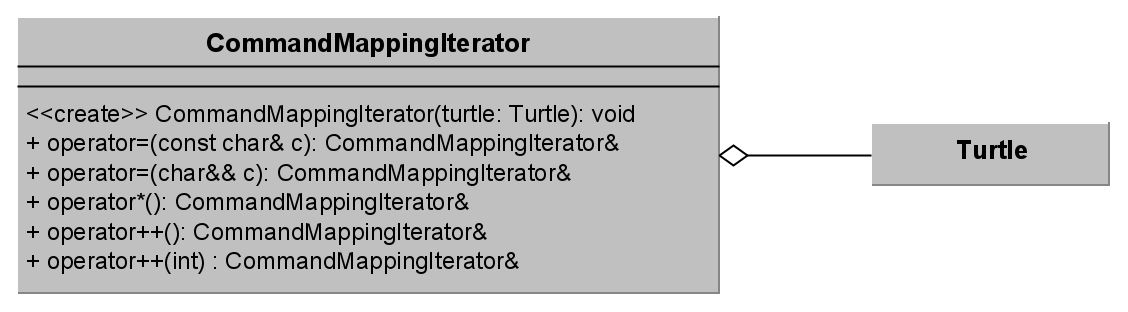
\includegraphics[width=1\columnwidth]{../graphs/LSystem/examples/class_command_mapping_iterator.png}
	\caption{Interface command mapper}
	\label{figure:if_command_map}
\end{figure}

The recursive function will receive this iterator as parameter and just hands the result over to the iterator. The command mapping just has to select the correct command and call it.
The indirection in form of the command mapper offers a clear separation between the calculation of the L-system generation and the handling of the data. In order to offer different mappings, new implementations of the iterator are nessecary. In the implementation, in section \ref{section:impl}, there is a simple implementation of the iterator based on the grammar introduced in previous sections.


\subsection{Configuration}
Some of the discussed components in this paper can be configured. The configuration could either be done in code, for example by setting it with constants, or in a dynamic way. A dynamic way would be possible by loading the configuration data from a stream, for example a filestream.
For the configuration of the introduced components it is sufficient to use simple key value pairs. For example such file could contain the configuration of a L-system:

\medskip

generations 14

axiom X

rule X YF+XF+Y

rule Y XF-YF-X

\medskip

\noindent In this example the key is seperated by the value with a space and in each row there is another key value pair. A problem is, that a value can not only consist of a single value, but can instead have of multiple values. For example a rule can consist of a precessor and a successor value. 
A solution for the multi value problem could be the use of a JSON object. A JSON object would allow to encapsulate the values without a restriction, but for this paper a simpler approach should be sufficient. As solution for the multi value objects is a simple separation of the values with a space. This is already shown in the example above, where a rule is splitted into three values.
When reading the data from a stream it is necessary to know what datatype the values have and therefore a mapping between the keys and the value type is needed. This can be done by a static mapping in the code, which will also allow to solve this in a flexible way. At least so flexible that the mapping can be set in a central place at the code.

\footnote{Hier muss man noch das genaue design beschrieben -> wie werden die daten übergeben bzw wie werden die daten gehalten oder werden die daten direkt übergeben }

\subsection{Overview}
This section will now give a short overview of the disscuessed components and their dependencies. The general approach for the design was a flexible use of the separated components. It should be possible to use each component on their own and even exchange a component and still guarantee the functionlity. Under the premises, that exchanged components still offer the same functionality and data. In figure \ref{figure:overview} a simplified overview of the dataflow is illustrated. 

\begin{figure}[h!]
	\centering
	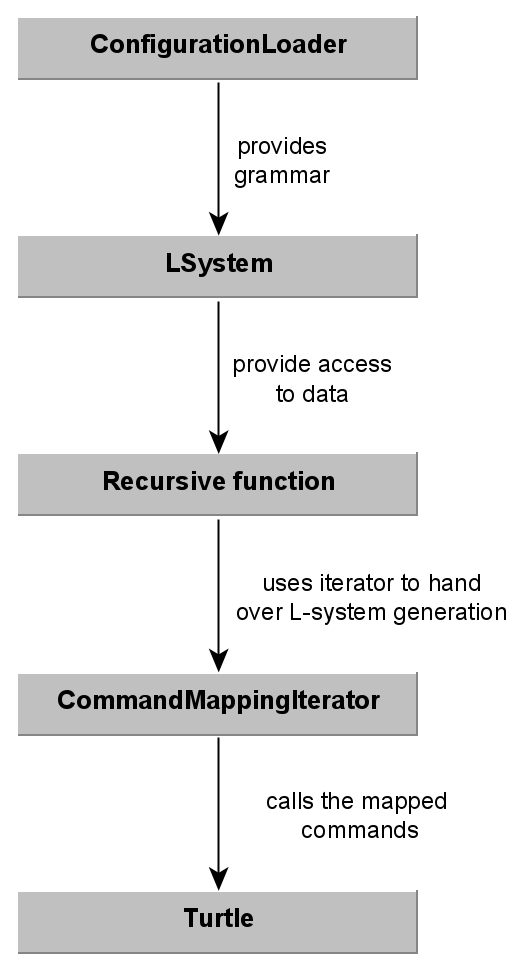
\includegraphics[width=0.4\columnwidth]{../graphs/LSystem/examples/overview.png}
	\caption{Simplified overview over the data flow}
	\label{figure:overview}
\end{figure}

\footnote{Configuration loader beschreiben}

The loaded data will be used to initalize the L-system. The L-system itself needs only to hold the grammar and and provide the access to it. The core of the L-system functionality is the recursive function, which will be used to calculate a L-system generation. This function offers a quiet flexible interface, because it should allow to use different L-system implementations, as long as the implementation provides a set of needed functions. These functions will be discussed in detail in section \ref{section:impl}. 
Another key part of the recursive function is the support of an arbitrary output iterator to hand over the calculated generation. This introduces not only a flexible usage of the function itself, but integrates well with already existing containers. 

The CommandMappingIterator is such an output iterator, which allows to use the provided interfaces to call the correct turtle command. Whenever data is handed over form the recursive function to the iterator, the iterator looks the data up and calls, if specified, the turtle command. The iterator here is  implemented for a determined mappping, but can be replaced by another implementation, as long as the implementation provides the typical output iterator functionality.

The final component is the turtle, which is used as abstract interface. This interface enforces the absolut minimal set of functions a turtle has to fullfill. Each spezialisation of a turtle has to independent handle their configuration and additonal dependencies.

As conclusion all the components can be exchanged with other objects, as long as they provide the needed interfaces. The needed interfaces will be described in detail in section \ref{section:impl} and addtional there are comments in the provided code.

\pagebreak

\section{Implementation}
\label{section:impl}
This section provides the in detail description of the implementation for the components discussed in the previous sections. Addtional to the components other aspects of the implementation, like the build system are discussed.

\subsection{Build System}
\label{section:buildsystem}
The first important point for the implementation is the question what build system to choose or if a build system is even needed. A build system is needed or at least comfortable to use  because of two points. The first point is a fast way to build a complexer design and even extend it with libraries in a fast way. The second point is the use on different operating systems, which also plays a big role for the question what build system to choose.
 
A typical build system for C++ projects are Makefiles, which include a description what and how to build. The problem with Makefiles is the restricted support on Windows, which results in either an inconvenient setup or to choose another build system.
In this context CMake comes to mind, a generator for buildsystems. It is possible to define the project in a file and CMake can generate files for different build systems, on different operating systems. These resolves not even the problem with the use of Windows, but enables other developers to build it on the system their choice.



TODO: SETUP FOR THIS PROJECT
PROBLEMS WITH WINDOWS -> DLLs



\subsection{ConfigurationLoader}

\subsection{LSystem}

\subsection{Recursive function}

\subsection{CommandMappingIterator}

\subsection{TurtleGraphic}
\subsubsection{TestTurtle}
\subsubsection{CairoTurtle}
\subsubsection{Further implementations}
SVG implementation


\section{Tests}
\section{Example usage}
\section{Problems and Restrictions}
\section{Outlook}

\footnote{FÜR ALLE UMLS DIE MEMBER VARIABLEN UM DEN UNTERSTRICH ERGÄNZEN}
\footnote{\fullcite{prusinkiewiczp.lindenmayera.2004}}
\end{document}